\documentclass[a4paper]{report}
\usepackage[utf8]{inputenc}
\usepackage[portuguese]{babel}
\usepackage{indentfirst}
\usepackage{hyperref} % \href
\usepackage{graphicx} % \includegraphics
\usepackage{float}
\usepackage{caption}
\usepackage{subfig}

\hypersetup{pdftitle={Report 1},
pdfauthor={Ariana Lousada, Carlos Gomes, Márcia Teixeira, Tiago Sousa},
colorlinks=true,
urlcolor=blue,
linkcolor=black}

\begin{document}

\title{Fase 1 \break
\large Grupo Nº 17}
\author{Ariana Lousada (A87998) \and Carlos Gomes (A77185) \and Márcia Teixeira (A80943) \and Tiago Sousa (A67674)}

\begin{center}
    \begin{minipage}{0.75\linewidth}
        \centering
        
\includegraphics[width=0.5\textwidth]{images/logo.png}\par\vspace{1cm}
        \vspace{1cm}
        \href{https://www.uminho.pt/}
        {\color{black}{\scshape\LARGE Universidade do Minho}}\par\vspace{1cm}
        \href{https://www.di.uminho.pt/}
        {\color{black}{\scshape\Large Departamento de Informática}} \par
        \maketitle
    \end{minipage}
\end{center}

\begin{figure}[H]
  \centering
  \begin{minipage}[b]{0.2\textwidth}
    \centering
    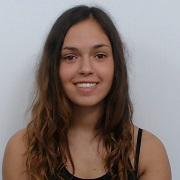
\includegraphics[width=\textwidth]{images/ariana.jpg}
    \caption*{Ariana Lousada (A87998)}
  \end{minipage}
  \hfill
  \begin{minipage}[b]{0.2\textwidth}
    \centering
    
\includegraphics[width=\textwidth]{images/carlos.png}
    \caption*{Carlos Gomes (A77815)}
  \end{minipage}
  \hfill
  \begin{minipage}[b]{0.2\textwidth}
    \centering
    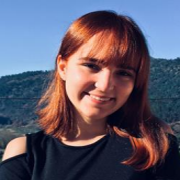
\includegraphics[width=\textwidth]{images/marcia.png}
    \caption*{Márcia Teixeira (A80943)}
  \end{minipage}
  \hfill
  \begin{minipage}[b]{0.2\textwidth}
    \centering
    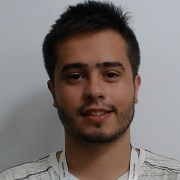
\includegraphics[width=\textwidth]{images/tiago.jpg}
    \caption*{Tiago Sousa (A67674)}
  \end{minipage}
  
\end{figure}

\tableofcontents

\pagebreak

\chapter{Introdução}
No âmbito da Unidade Curricular de Desenvolvimento de Sistemas de Software, foi-nos proposto a realização de um trabalho prático que visa a criação de um sistema de gestão de \textit{stocks} de um armazém de uma fábrica.

Com este relatório temos o objectivo de apresentar a modelação do projecto da unidade curricular de Desenvolvimento de Sistemas de Software. Nesta primeira fase, iremos abordar nomeadamente dois tipos de modelação: Modelagem de Domínio e de \textit{Use Cases}.\\

Apesar de existir alguma flexibilidade em relação ao modo de operação do sistema, este mesmo deve obedecer um conjunto de critérios previamente estabelecidos e que iremos explorar ao longo do projecto.

\chapter{Modelo de Domínio}
O modelo de domínio ilustra as classes conceptuais significativas no domínio do problema. Sendo assim, este modelo irá conter todas as entidades envolvidas no sistema e ao mesmo tempo o relacionamento entre eles.

Para elaborarmos um modelo de domínio, primeiro devemos identificar as entidades e então estabelecer os relacionamentos entre elas, finalmente definimos as multiplicidade das entidades envolvidas em cada relacionamento.

Neste capítulo serão apresentados os pontos chave do problema assim como uma proposta de Modelo de Domínio inicial para tentar responder ao problema.
 
\section{Descrição de Modelo de Domínio} 
O enunciado consiste em desenvolver um sistema de gestão de armazenamento de materiais num armazém com recurso a robots. Este sistema automatizado é responsável pela gerência do inventário do armazém, mantendo actualizado o seu estado de lotação, com o auxílio de robots automatizados, responsáveis pela organização do mesmo. \\
Após análise do enunciado, concluímos que necessitamos dos seguintes:
\begin{enumerate}
    \item \textbf{Sistema} - Esta entidade é o foco principal deste projeto, controlando a maior parte dos processos que consideramos essenciais, tais como, pedidos de descarga/acesso, manutenção de queues(de entrega e de espera), mapeamento do armazém e respetivas rotas que são por sua vez distribuídas pelos robots. \newline
    \item \textbf{Robots} - São responsáveis pelo correto armazenamento e organização do inventário, dadas as rotas calculadas. \newline
    \item \textbf{Inventário} - Informação necessária, relativa aos produtos existentes no armazém (número de prateleira, secção, QR-Code, etc). \newline
    \item \textbf{Armazém} - Espaço físico, gerido pelo sistema, com o objetivo de armazenar as matérias primas que são entregues, que por sua vez são recebidas na zona de entregas. O armazenamento encontra-se dividido em: \textit{Zona Refrigerada} e \textit{Zona não refrigerada}. \newline
    \item \textbf{Materiais} - Encontram-se organizados em paletes, que são posteriormente armazenadas pelos robots, que as organizam consoante o seu tipo: \textit{perecíveis}(em zonas refrigeradas) ou \textit{não perecíveis}(em zonas não refrigeradas). \newline
    \item \textbf{Utilizador} - Entidade externa ao sistema que possui acesso a este para dele usufruir. Esta entidade pode ser um \textit{Gestor} ou um \textit{Encarregado}, que vai atualizando o inventário. \newline
    \item \textbf{Gestor} - Utilizador que controla os materiais que entram no armazém (com auxílio do \textit{Leitor de QR-Code}). Também aceita/rejeita pedidos de entrega feitos pelos motoristas. \newline
    \item \textbf{Encarregado} - Utilizador responsável pelos materiais que saem do armazém (com auxílio do \textit{Leitor de QR-Code}). Também aceita/rejeita pedidos de requisição de materiais e notifica o sistema adequadamente. \newline
    \item \textbf{Servidor de Produção}  - Realiza requisições de materiais que são posteriormente aceites/rejeitadas pelos \textit{Encarregados}.
\end{enumerate}

\section{Representação do Modelo de Domínio}

\begin{figure}[H]
\begin{center}
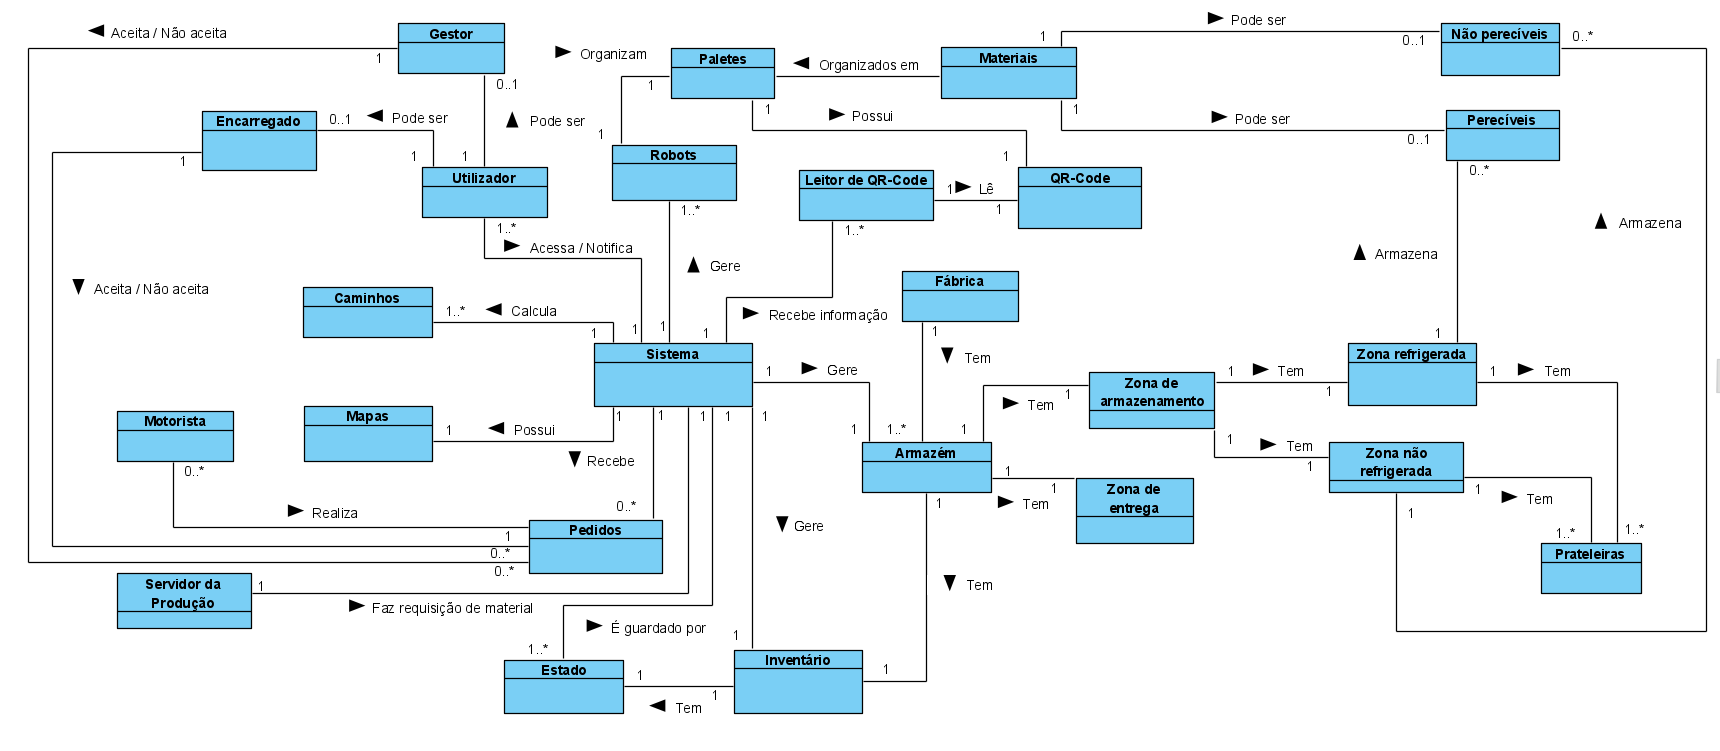
\includegraphics[scale=0.40]{images/MD.png}
\caption{\label{fig:MD} Modelo de Domínio }
\end{center}
\end{figure}

\chapter{Use Cases}

Este tipo de modelagem incide mais nas entidades externas ao sistema, descrevendo como este interage com o seu ambiente. Essas interações são representadas como casos de uso (isto é,\textit{Use Cases}) que descrevem como os diferentes Atores (objetos externos) se interligam com o sistema em causa em diferentes cenários.

\section{Actores}
Os actores aqui referidos têm cada um interações essenciais ao sistema, que permitem o seu constante funcionamento:
\begin{itemize}
    \item \textbf{1} : Motorista
    \item \textbf{2} : Leitor de QR-Code
    \item \textbf{3} : Servidor de Produção
    \item \textbf{4} : Robots
    \item \textbf{5} : Utilizador
    \item \textbf{6} : Gestor
    \item \textbf{7} : Encarregado
\end{itemize}

\pagebreak

\section{Funcionamento do armazém}
Tal como foi referido anteriormente, o sistema desenvolvido neste projeto envolve um armazém, na qual se faz a organização de \textit{stocks}. Este pode ser consultado por um \textbf{Utilizador}, caso este deseje algum tipo de informação relativa ao armazém, como por exemplo: listagens de produtos presentes no estabelecimento, produtos presentes nas queues (de entrega e de espera), entre outros.

Para isto, o \textbf{Motorista} solicita uma autorização para descarga de materiais, que é processada pelo sistema. Conforme a disponibilidade do armazém, o \textbf{Gestor} autoriza/não autoriza a descarga.

Com isto, o \textbf{Leitor de QR-Code} lê os códigos das paletes entregues. Essa informação é posteriormente comunicada ao sistema, de modo a que este seja capaz de atualizar o seu inventário, assim como uma notificação que é enviada pelo \textbf{Gestor}.

De seguida, são solicitados \textbf{Robots} automatizados para armazenarem as paletes de acordo com a localização e caminho que lhes são atribuídos pelo sistema (de acordo com o tipo de material que as compõem). Cada um destes \textbf{robots} possui um estado, que pode ser \textit{disponível} ou \textit{indisponível}. Apenas os robots disponíveis são notificados para o armazenamento, que por sua vez notificam o sistema quando terminam o transporte.

Este armazém assim como recebe materiais através dos \textbf{Motoristas}, o \textit{Servidor de produção} também pode solicitar requisições de materiais, que são também aceites pelo sistema de acordo com a sua disponibilidade.

Para além disto, o sistema também é capaz de retirar produtos do armazém. Essa saída é monitorizada pelo \textbf{Encarregado}, que envia uma notificação sempre que há materiais que saem do estabelecimento. O transporte das paletes é também neste caso feito pelos \textbf{Robots}.

% \ref{appendix:a1}

\newpage

\pagebreak
\section{Representação do Diagrama de Use Case}

\begin{figure}[H]
\begin{center}
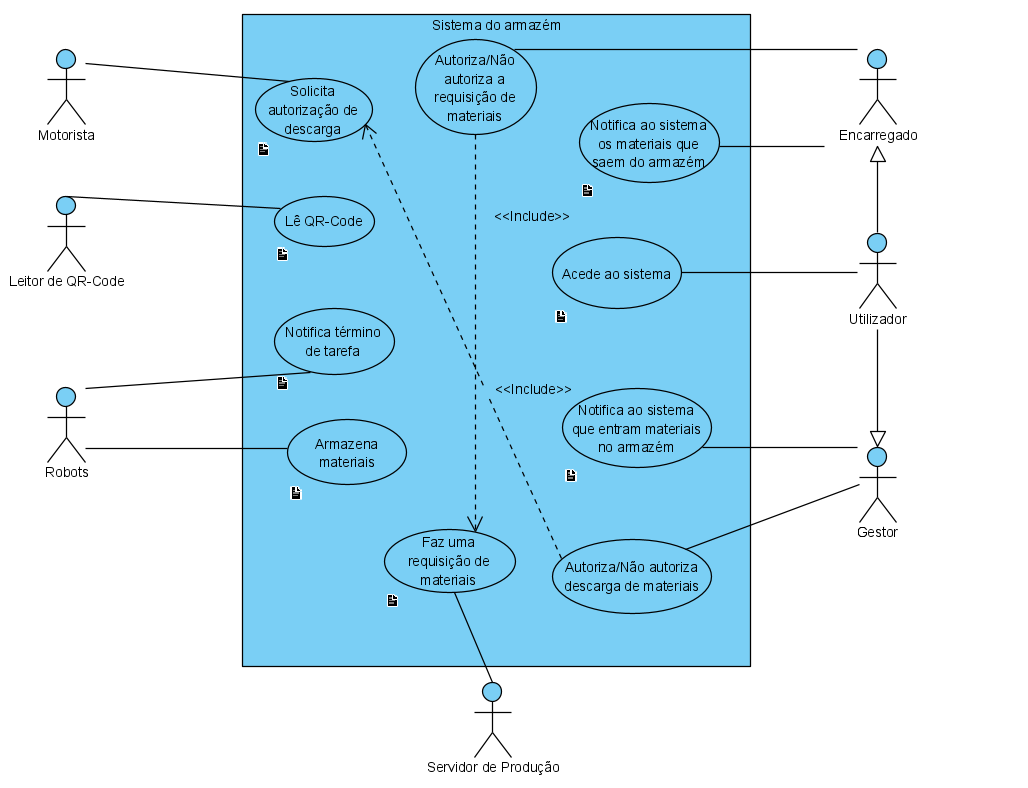
\includegraphics[scale=0.60]{images/UC.PNG}
\caption{\label{fig:UC}Representação do diagrama de Use Case}
\end{center}
\end{figure}

\chapter{Conclusão}
Através da realização desta primeira etapa do trabalho conseguimos melhor perceber como o planeamento e modelação de um programa são importantes.\\

Este planeamento e modelação de domínio permitiu-nos uma melhor percepção do problema que nos foi apresentado.\\
Por sua vez o diagrama de use cases apresentou-nos uma boa ideia sobre como, numa fase futura, poderemos desenvolver as funcionalidades básicas da nossa aplicação, assim como as entidades que irão interagir com ela.\\

Isto tudo irá-nos ajudar a desenvolver a parte do código deste projeto com uma maior organização e destreza, melhorando a sua qualidade assim como a sua interpretação.\\

\appendix
\chapter{Descrição de Use Cases}
\label{appendix:a1}


% Caso 1
\section{Solicita autorização de descarga}

\textbf{Use Case:} Solicita autorização de descarga

\textbf{Actores:} Motorista

\textbf{Descrição:} O motorista faz um pedido de descarga de matérias no armazém 

\textbf{Pré-condição:}  O armazém tem espaço disponível.

\textbf{Pós-condição:} Os materiais são entregues e colocados na zona de entrega

\textbf{Fluxo Normal:} 
\begin{enumerate}
    
    \item  O sistema recebe o pedido de descarga 
    \item O gestor acede ao sistema e autoriza o motorista 
    \item Os materiais são colocados na zona de entregas
\end{enumerate}

\textbf{Fluxo de excepção 1: [Não há espaço disponível no armazém]} 

\begin{enumerate}

    \item  O gestor não autoriza a entrega. 
    \item Os materiais não são entregues. 

\end{enumerate}

% Caso 2
\newpage

\section{Lê o QR-Code}

\textbf{Use Case:} Lê o QR-Code

\textbf{Actores:} Leitor de QR-Code

\textbf{Descrição:} O leitor lê o código do material e o sistema adiciona o produto ao inventário 

\textbf{Pré-condição:}  Existem produtos a adicionar ao sistema.

\textbf{Pós-condição:} A informação do novo produto é adicionada ao inventário do armazém.

\textbf{Fluxo Normal:} 
\begin{enumerate}

    \item  O leitor regista o QR-Code e envia a informação necessária ao sistema. 
    \item O sistema regista o material juntamente com o QR-Code no inventário do armazém.

\end{enumerate}

\textbf{Fluxo de excepção 1: [Não existem produtos para registar]} 

\begin{enumerate}

    \item  O leitor fica em stand-by (fica temporariamente desativado).
\end{enumerate}


% Caso 3
\newpage

\section{Faz uma requisição de materiais}

\textbf{Use Case:} Faz uma requisição de materiais

\textbf{Actores:} Servidor de Produção

\textbf{Descrição:} O servidor faz uma requisição de materiais  

\textbf{Pré-condição:} True

\textbf{Pós-condição:} Os materiais pedidos são pedidos e colocados na queue de entregas.

\textbf{Fluxo Normal:} 
\begin{enumerate}
    \item O servidor solicita lista de paletes.
    \item O sistema verifica que ainda existe espaço no armazém.
    \item O sistema acede ao inventário e confirma a disponibilidade das paletes pedidas.
    \item A requisição é comunicada ao sistema.
    \item O encarregado verifica a requisição e notifica o sistema. 
\end{enumerate}

\textbf{Fluxo Alternativo 1: [O armazém não tem espaço suficiente] (Passo 2)}
\begin{enumerate}
    \item [2.1.] A requisição não é solicitada.
\end{enumerate}
     
\textbf{Fluxo Alternativo 2: [Algumas paletes estão indisponíveis] (Passo 3)}
\begin{enumerate}
    \item [3.1.] Sistema informa quais são as paletes indisponíveis.
    \item [3.2.] Servidor confirma o pedido completo.
    \item [3.3.] Sistema solicita a requisição.
    \item [3.4.] As paletes pedidas são colocadas na queue de entregas.
    \item [3.5.] As paletes em falta são colocadas na queue de espera.
\end{enumerate}

\textbf{Fluxo Alternativo 3: [O encarregado só quer as paletes existentes] (Passo 3.2)}
\begin{enumerate}
    \item [3.2.1.] O servidor confirma o pedido só das paletes existentes.
    \item [3.2.2.] As paletes disponíveis são colocadas na queue de entregas.
\end{enumerate}
    
\textbf{Fluxo de exceção 1: [O encarregado quer cancelar o pedido] (Passo 3.2)}
\begin{enumerate}
    \item [3.2.1.] O servidor cancela o pedido.
\end{enumerate}
    

% Caso 4
\newpage

\section{Notifica término de tarefa}

\textbf{Use Case:} Notifica término de tarefa

\textbf{Actores:} Robot

\textbf{Descrição:} O robot notifica o sistema quando termina o armazenamento de uma palete. 


\textbf{Pré-condição:}  O robot arrumou uma palete com sucesso.

\textbf{Pós-condição:} O sistema recebe a notificação 

\textbf{Fluxo Normal:} 
\begin{enumerate}

    \item O robot arruma uma palete no local designado.
    \item O robot notifica o sistema.
    \item O sistema recebe a notificação e coloca o estado do robot como livre.

\end{enumerate}

\textbf{Fluxo de Exceção 1: [O robot não consegue terminar a tarefa]}
\begin{enumerate}
    \item O sistema notifica os utilizadores de que algo correu mal.
\end{enumerate}



% Caso 5
\newpage

\section{Armazena materiais}

\textbf{Use Case:} Armazena materiais

\textbf{Actores:} Robot

\textbf{Descrição:} Os robots armazenam materiais  


\textbf{Pré-condição:}  Existem materiais na zona de entrega.

\textbf{Pós-condição:} Os materiais ficam armazenados no armazém e registados no sistema.

\textbf{Fluxo Normal:} 
\begin{enumerate}

    \item  O sistema verifica os robots disponíveis e seleciona-os para armazenamento.
    \item O sistema calcula caminhos para cada robot utilizado e distribui-os adequadamente.
    \item Os robots armazenam os materiais.

\end{enumerate}

\textbf{Fluxo Alternativo 1: [Não existem robots disponíveis para o trabalho] (Passo 1)}
\begin{enumerate}
    \item [1.1.] Espera que um robot complete a tarefa atual.
    \item [1.2.] Sistema coloca o robot como disponível.
    \item [1.3.] Volta ao passo 2.
\end{enumerate}


\textbf{Fluxo Alternativo 2: [N robots obtêm caminho igual] (Passo 2)}
\begin{enumerate}
    \item [2.1.] O sistema analisa os caminhos em causa.
    \item [2.2.] Escolhe (n-1) robots aleatoriamente e utiliza diferentes "áreas" do mapa para calcular novos caminhos.
    \item [2.3.] Volta a distribuir os caminhos novos aos robots em causa.
    \item [2.4.] Volta ao passo 4.
\end{enumerate}

\textbf{Fluxo de Exceção 1: [Não existem paletes para armazenar]}
\begin{enumerate}
    \item Os robots acabam as tarefas atuais e aguardam por novas ordens.
\end{enumerate}



% Caso 6
\newpage

\section{Acede ao sistema}

\textbf{Use Case:} Acede ao sistema

\textbf{Actores:} Utilizador

\textbf{Descrição:} O utilizador acede ao sistema 

\textbf{Pré-condição:}  True

\textbf{Pós-condição:} O utilizador obtém a informação que pede.

\textbf{Fluxo Normal:} 
\begin{enumerate}

    \item  O utilizador acede ao sistema.
    \item O utilizador pede a informação que pretende ter acesso.
    \item O sistema disponibiliza essa mesma informação ao utilizador.

%Caso 7
\newpage

\section{Notifica ao sistema os materiais que saem do armazém}

\textbf{Use Case:} Notifica ao sistema os materiais que saem do armazém

\textbf{Actores:} Encarregado

\textbf{Descrição:} O encarregado notifica o sistema quando saem paletes do armazém.

\textbf{Pré-condição:} O encarregado envia uma notificação para informar o sistema que uma ou mais paletes saíram do armazém.

\textbf{Pós-condição:} O sistema recebe a notificação.

\textbf{Fluxo Normal:} 
\begin{enumerate}

    \item A(s) palete(s) é(são) selecionada(s) para saírem do armazém.
    \item O encarregado notifica o sistema.
    \item O sistema recebe a notificação e retira a(s) palete(s) do inventário do armazém.
\end{enumerate}

%Caso 8
\newpage

\section{Notifica ao sistema que entram materiais no armazém}

\textbf{Use Case:} Notifica ao sistema que entram materiais no armazém

\textbf{Actores:} Gestor

\textbf{Descrição:} O gestor notifica o sistema quando entram paletes do armazém.

\textbf{Pré-condição:} O encarregado envia uma notificação para informar o sistema que uma ou mais paletes saíram do armazém.

\textbf{Pós-condição:} O sistema recebe a notificação.

\textbf{Fluxo Normal:} 
\begin{enumerate}

    \item A(s) palete(s) entram no armazém.
    \item O gestor notifica o sistema.
    \item O sistema recebe a notificação e aguarda informação do leitor de QR-Code.
\end{enumerate}

\end{enumerate}
\end{document}